\section{結論}

本次專題,使用Duckietown之虛擬城市環境,設計小型探測車裝置,並開發影像辨識與定位之功能,從而瞭解系統運作原理以及學習使用定位與影像辨識之技術。本學期已達成物件辨識與定位之功能,未來希望能加入Lidar與編碼器馬達之SLAM技術,進行更準確之定位與搜救平台研究開發。

\begin{figure}[bht]
	\centering
	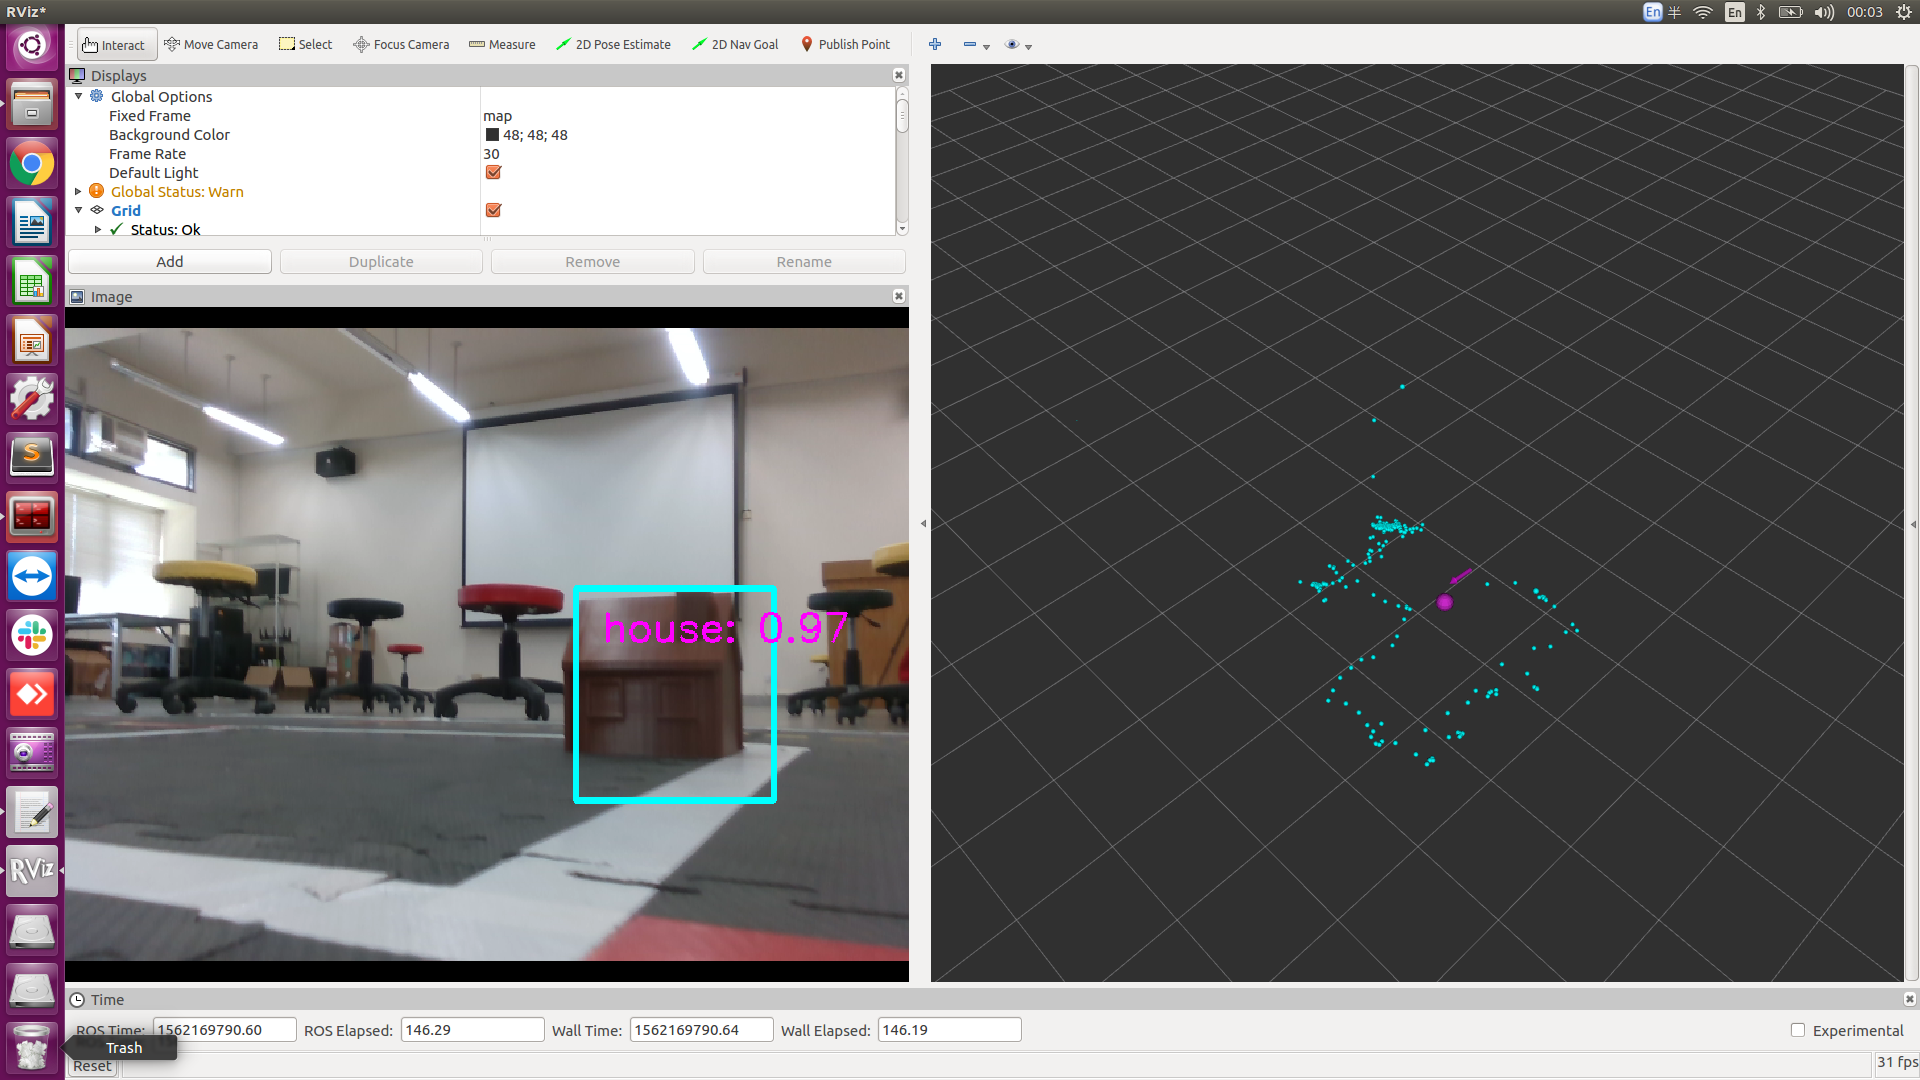
\includegraphics[width=\linewidth,keepaspectratio=true]
	{images/demo.png}
	\caption{專題成果呈現}
	\label{figure:localization_result}
\end{figure}
